\documentclass{article}

\usepackage{fullpage}
\usepackage{tikz}

\newcommand{\creategrid}[2]{%
  \draw[step=1] (0,0) grid (#1,#2);%
%
  \foreach \x in {1,...,#1}%
    \draw (\x - 0.5, -0.5) node {\x};%
%
  \foreach \y in {1,...,#2}%
    \draw (-0.5, \y - 0.5) node {\y};%
}%
\newcommand{\drawobstacle}[2]{%
\draw[fill=black] (#1,#2) rectangle +(-1,-1);
}%


\begin{document}

\title{Block Jump Point Search}
\maketitle

\begin{abstract}
  This document gives some ideas for improving Jump Point Search (JPS) 
  by manipulating ``blocks'' of grid nodes rather than individual nodes.  
  It is our intuition that such techniques 
  will improve the performance of JPS for two reasons: 
  i) it will reduce the number of operations 
  (a group of nodes will be processed in one go); 
  ii) it will reduce the number of cache misses 
  (by manipulation pieces of data that are adjacent in memory).  
\end{abstract}

\section{Data Structure}

A first idea is to store the grid 
so as to minimise the distance between the places in memory 
that store information for two consecutive requests.  
Consider the jump point search problem 
on Figure~\ref{fig::grid} (this is only part of the grid; 
it is assumed that the grid extends very far on each of the four sides) 
where the node $N = \langle 2,4\rangle$ is expanded 
coming from node $P = \langle 1,3\rangle$.  
%More precisely, we would like to maximise the number of situations 
%where the piece of information 
%for the current request 
%is on the same block of information 
%as some very recent request.  
%Ideally the information would be in the same processor register.  
%As a consequence, no cache miss occurs for accessing this information.  

\begin{figure}[ht]
  \begin{center}
    \scalebox{0.8}{%
      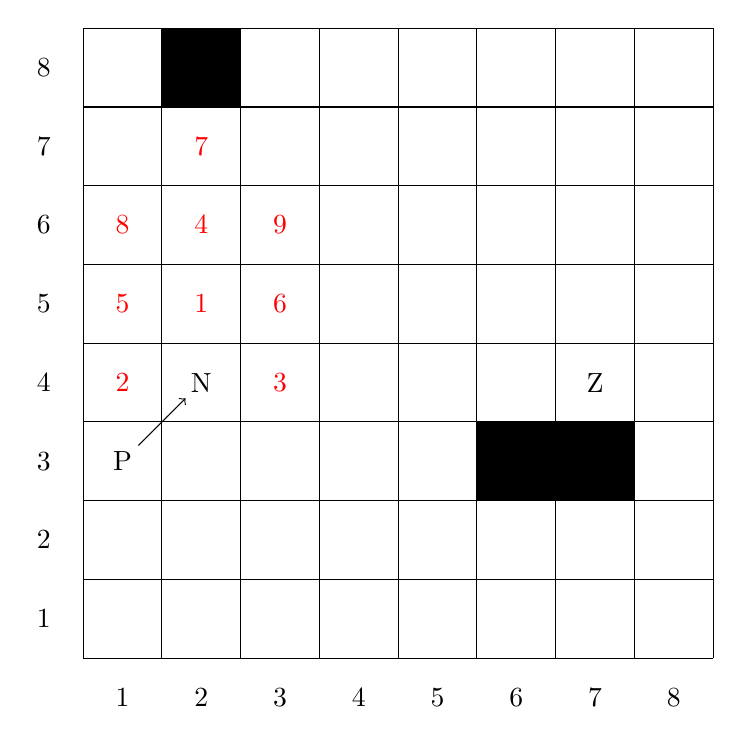
\begin{tikzpicture}
        \creategrid{8}{8}
        \drawobstacle{2}{8}
        \drawobstacle{7}{3}
        \drawobstacle{6}{3}
        \draw[->] (0.7,2.7) -- (1.3,3.3);
        \draw (1.5,3.5) node {N};
        \draw (0.5,2.5) node {P};
        \draw (6.5,3.5) node {Z};
        \draw (1.5,4.5) node[red] {1};
        \draw (0.5,3.5) node[red] {2};
        \draw (2.5,3.5) node[red] {3};
        \draw (1.5,5.5) node[red] {4};
        \draw (0.5,4.5) node[red] {5};
        \draw (2.5,4.5) node[red] {6};
        \draw (1.5,6.5) node[red] {7};
        \draw (0.5,5.5) node[red] {8};
        \draw (2.5,5.5) node[red] {9};
      \end{tikzpicture}%
    }
  \end{center}
  \caption{A current search state 
    (the grid is assumed larger than the part presented).}
  \label{fig::grid}
\end{figure}

At this stage, we have to check 
whether there is a node with a forced neighbour on column $2$ from $N$ 
and similarly for row $4$ (in this instance, there is: $Z$).  
In this example, the presence of an obstacle 
will be verified (more or less) in the order given in red on the figure.  
Essentially, three columns are explored in parallel.  
A trivial representation of the grid as a one or two dimensional array
would put node $1$ far away from node $2$ in memory.  
What we propose is to put the information for node $1$ and $2$ 
in the same 32 bit- (or 64 bit-) register.  
Technically, one integer would represent the rectangle 
from $\langle 1,1\rangle$ to $\langle 4,8\rangle$.  
There are two issues here: 
\begin{itemize}
\item 
  In the example given above, we explore the column 2, 
  and the integer contains the information in columns 1--4 
  (which is convenient).  
  If we are to explore the column 4, 
  then we need information from columns 3, 4, and 5, 
  hence from two different integers.  
  We could have two copies of the grid: 
  a rectangle from $\langle 1,1\rangle$ to $\langle 4,8\rangle$ 
  and a rectangle from from $\langle 3,1\rangle$ to $\langle 6,8\rangle$.  
\item 
  We want the rectangle to be long and not large, 
  so that we can search far without loading a new rectangle.  
  We might also want another copy of the grid for when we explore rows
  rather than columns.
\end{itemize}
A number of these possibilities require increased memory overheads. 
We would need experiments to decide the best option. For example
For example, how large should we make our rectangles? How much benefit can we
derive from storing two copies of the map, one ordered by rows and the other
orderd by columns? Does overlapping rectangles yield a substantial
performance gain over the above?

\section{Empty Blocks}

Consider again the example given in Figure~\ref{fig::grid}.  
Assume now that there is no obstacle in $\langle 2,8\rangle$.  
Rather than testing every grid node individually, 
we could immediately (i.e., virtually for free) determine 
that the integer representing the rectangle 
evaluates to $0$, i.e., there is no obstacle.  
Because there is no obstacle in the rectangle, 
we can immediately jump to the next rectangle.  

\section{Identifying Jump Point in Non Empty Blocks}

The idea here is to use bitwise operators
to manipulate a bunch of nodes together.  
Consider the left-to-right exploration of row $4$.  
The following bytes (bytes are used for simplicity; 
the idea generalises to blocks of any size, e.g., integers) 
represent the obstacles in rows 5, 4, and 3.  

\begin{center}
  \begin{tabular}{|c|c|c|c|c|c|c|c|}
    \hline
    0 & 0 & 0 & 0 & 0 & 0 & 0 & 0 \\
    \hline
    0 & 0 & 0 & 0 & 0 & 0 & 0 & 0 \\
    \hline
    0 & 0 & 0 & 0 & 0 & 1 & 1 & 0 \\
    \hline
  \end{tabular}
\end{center}

We want to identify (i) the positions $x$ on row~4 which are traversable and can
be reached without hitting an obstacle and (ii) the positions $x$ which have
forced neighbours at locations $x-1$ in rows $3$ or $5$.
For instance, to decide which positions $x$ from row 3 
are not obstacles, you simplify need to do a bitwise negation: 
\begin{center}
  \begin{tabular}{|c|c|c|c|c|c|c|c|}
    \hline
    1 & 1 & 1 & 1 & 1 & 0 & 0 & 1 \\
    \hline
  \end{tabular}
\end{center}
To decide the positions $x$ on row 3 
such that there is an obstacle on position $x-1$, 
you simplify need to do a shift: 
\begin{center}
  \begin{tabular}{|c|c|c|c|c|c|c|c|}
    \hline
    0 & 0 & 0 & 0 & 0 & 0 & 1 & 1 \\
    \hline
  \end{tabular}
\end{center}
To decide the positions $x$ on row 3 
that satisfy both property defined above, 
you simplify need to do a bitwise \& operation 
on the two last bytes: 
\begin{center}
  \begin{tabular}{|c|c|c|c|c|c|c|c|}
    \hline
    0 & 0 & 0 & 0 & 0 & 0 & 0 & 1 \\
    \hline
  \end{tabular}
\end{center}

Deciding whether the first jump point is  reached
before an obstacle is hit on the current row 
could probably be tested by a $\le$ operation or via
some bit masking mechanism.
Clearly, details need to be worked out here but the problem
is cute and looks fun to solve.

\section{Preprocessing}
One straightfoward approach to speeding up JPS is to preprocess
the entire map and replace the neighbours of each node
with the first jump point that can be reached by travelling in the
direction of each neighbour. A sketch of this idea has been 
outlined already~\cite{harabor12}.
Preprocessing eliminates entirely the need to search for jump
points but it has two disadvantages (i) jump points need to be recomputed
if the map changes (some local repair seems enough) and (ii) it introduces 
a substantive memory overhead: we need to keep for each node 8 distinct identifiers. 
The overhead can be as large as $4\times8$ bytes per node.

A more memory efficient approach is to store just 2 or 3 bits for each
of the cardinal neighbours (north, south, east, west).
The value indicates how many steps we can take before 
reaching a jump point (0 if no jump point exists). We thus still
need to search but we only need to consider one row (or column) of 
the grid at a time. We can keep two copies of the map: one
which has the values for traveling north/south, one which
has the values for travelling east/west. 

\section{Waves}
The wave approach builds on previous bitwise ideas, 
but the details are rather different.  
I will give an example, again based on the figure.  

Assume that we are searching from somewhere in the bottom 
and that, from there, it has been proved 
that the shortest path to any node on row 2 
is through a combination of North-East moves followed by North moves.  
This knowledge is represented through the following byte: 
\begin{center}
  \begin{tabular}{|l|c|c|c|c|c|c|c|c|}
    \hline
    $r(2)$ & 1 & 1 & 1 & 1 & 1 & 1 & 1 & 1 \\
    \hline
  \end{tabular}
\end{center}
Byte $r(2)$ contains $1$s for the positions 
that can be reached with a combination of NE+E.  

How do we compute $r(3)$?  
That's pretty simple: $r(3)$ contains a $1$ at position $x$ 
iff $r(2)$ does and there is no obstacle at $\langle x,3\rangle$.  
This is a simple bitwise negation + bitwise \&.  
\begin{center}
  \begin{tabular}{|l|c|c|c|c|c|c|c|c|}
    \hline
    $grid(3)$  & 0 & 0 & 0 & 0 & 0 & 1 & 1 & 0 \\
    \hline
    $!grid(3)$ & 1 & 1 & 1 & 1 & 1 & 0 & 0 & 1 \\
    \hline
    $r(3) = r(2) \& !grid(3)$ & 1 & 1 & 1 & 1 & 1 & 0 & 0 & 1 \\
    \hline
  \end{tabular}
\end{center}

Now, we are interested in determining the positions 
where JPS might want to stop moving North-East and start moving North.  
This is represented by the $j$ byte: 
\begin{center}
  \begin{tabular}{|l|c|c|c|c|c|c|c|c|}
    \hline
    $j(2)$ & 0 & 0 & 0 & 0 & 0 & 0 & 0 & 0 \\
    \hline
  \end{tabular}
\end{center}
Here, we haven't identified any position 
where the agent should stop.  

For instance, the bits of position $5$ and $8$ 
should turn to $1$ in byte $j$ when we reach row $4$.  
This is identified by noting 
that there is an adjacent position $x'$ 
where there was an obstacle at row $3$ 
and there is no more obstacle at row $4$.  

Details need to be worked out, 
but the idea is that it can be implemented with bitwise operations.  

%\section*{Acknowledgments}
%\section{Acknowledgements}
\label{sec::ack}
We thank Patrik Haslum for taking the time to read and comment on 
an early revision of this paper.
NICTA is funded by the Australian Government through the Department of
Communications and the Australian Research Council through the ICT Centre of
Excellence Program.

\bibliographystyle{plain}
\bibliography{references}

\end{document}
